\section{Introduction}
%Will wrote this introduction - feel free to make changes, but please note the changes too!
The aim of this project was to create a model capable of predicting the sales using information available prior to the launch of a game.

A model capable of making accurate predictions based on several different input parameters would prove quite useful to game development studios trying to anticipate the market performance of a specific project. This model would then also allow said studios to design projects with a mindset of optimising profits. 

%Joe modified this section
The inputs for our model consisted of game information scraped off of the steam product page, this included the price of a game at launch, the genre of the game and whether the game offered additional features e.g. controller support or local multiplayer, under the label "Specs". The target values for our model was provided by

the SteamSpy API. This API provides an estimated range for the number of owners a games has at a 98\% confidence interval
LASSO, Ridge and kNN Regression were then trained to try and best predict the sales of the given game.

\section{Dataset and Features}

%Darragh's part
One of the datasets that we used for our model comes from the SteamSpy API. The most efficient way to obtain the data is to use a get request on the list of genres available. There are a total of 39230 games. Each game contains a number of features related to the game such as App ID, Name, Developer, Publisher, Number of positive reviews, Number of negative reviews, Average users and Price. The genre of the game was also manually added to this list by filtering the get requests by this parameter. This data is used in conjunction with the data retrieved from the scraper to create our finished dataset.

%Will's part
To generate the target feature (the number of sales), a number of features available from SteamSpy had to be manipulated to produce useful values. SteamSpy offered a range of owners to 98\% confidence, but did not offer a precise number of owners for a given game. In a bid to produce better approximations of title ownership, a method for making these approximations was created.

The total reviews for each ownership bracket (e.g. games with anywhere between 0-20,000 owners) were entered into a bracket-dependent row, and the entries of each row were normalised against the other entries of the row.

After the differing brackets had been normalised, these scaling parameters were then collected in an array, and each entry in the array was multiplied by the associated mean of the relevant bracket, to create a weighted distribution of owners. This increased the distinction between games lying in the same bracket, so that the model would no longer believe a game with 5 owners was as popular as a game with 19,000.

\section{Methods}
%Will's writing:
Three forms of model were used: LASSO, Ridge and kNN regression in a bid to find which models would best predict the target feature.

Both LASSO and Ridge regression are modifications of Linear regression, in that they each attribute different penalties to the cost functions used to fit their curves.

Taking the cost function of Linear regression to have the form:
\[
J(\theta) = \frac{1}{m} \sum_{i=1}^m (h_{\theta}(x^{(i)}) - y^{(i)})^2
\]

Then $J(\theta)$ for LASSO regression with its (L1) penalty becomes:
\[
J(\theta) = \frac{1}{m} \sum_{i=1}^m (h_{\theta}(x^{(i)}) - y^{(i)})^2 + \frac{1}{C} \sum_{j=1}^n |\theta_j|
\]
And $J(\theta)$ for Ridge regression with its (L2) penalty becomes:
\[
J(\theta) = \frac{1}{m} \sum_{i=1}^m (h_{\theta}(x^{(i)}) - y^{(i)})^2 + \frac{1}{C} \sum_{j=1}^n \theta_j^2
%\frac{\theta^T \theta}{C}
\]

k-Nearest Neighbours regression on the other hand defines weighting based on the proximity between nearby points to make predictions; rather than fitting an overall trend immediately, kNN looks at the local behaviours first to build up a picture of the system. It is in this way that the method is considered "instance-based".

\section{Results}

%Will's Part
The results of the investigation fell slightly short of expectations as both the standard and kernelised kNN methods required a prohibitive amount of time to train, preventing the collection of data from those models. %Hold your horses there chief - may be able to do something yet!

These setbacks aside, it was possible to investigate the performance of both the LASSO and Ridge regression methods, by way of mean squared error and $R^2$ value. Both of these models were trained for n=10 splits.
\vspace{8pt}

Figure \ref{fig:fig1} demonstrates some of the difficulty with using the LASSO approach for this problem. The MSE reaches a minimum that is below the baseline at C = $2^{16}$, where it also achieves the highest $R^2$ value of 0.1256. Regrettably, the variance of a number of points seems to nullify the utility of certain other data points.

\begin{figure}[!h]
\begin{small}
\centering
\linespread{1.0}
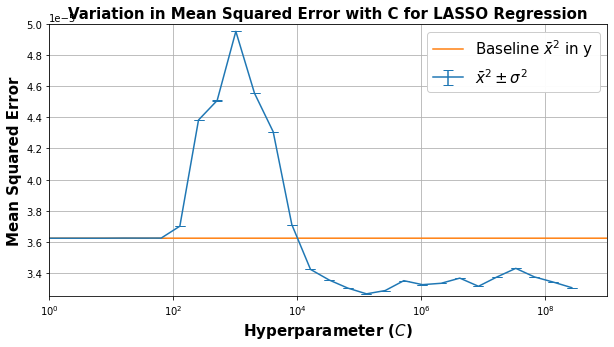
\includegraphics[width=0.8\linewidth]{pics/Lasso_MSE.png}
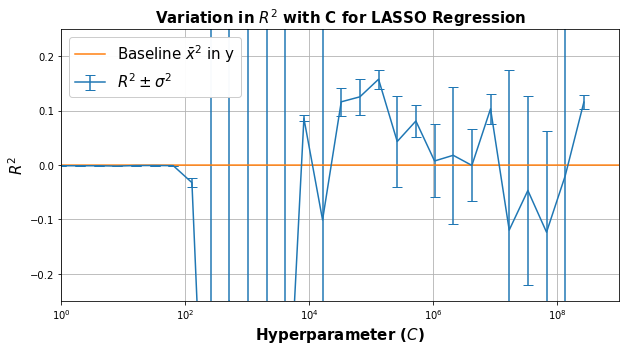
\includegraphics[width=0.8\linewidth]{pics/Lasso_R2.png}
\caption{Varying C eventually loweres the MSE, but has no consistent impact on $R^2$.}
\label{fig:fig1}
\end{small}
\end{figure}

\vspace{8pt}

Figure \ref{fig:fig2} shows the increased performance of Ridge regression over LASSO regression - MSE is consistently lower for Ridge Regression, and the optimal C according to MSE and $R^2$ appears at a much lower value of C = 0.03125. $R^2$ itself is about 0.127, so at this value of C, we can observe an improvement in Ridge regression over LASSO regression.


\begin{figure}[!h]
\begin{small}
\centering
\linespread{1.0}
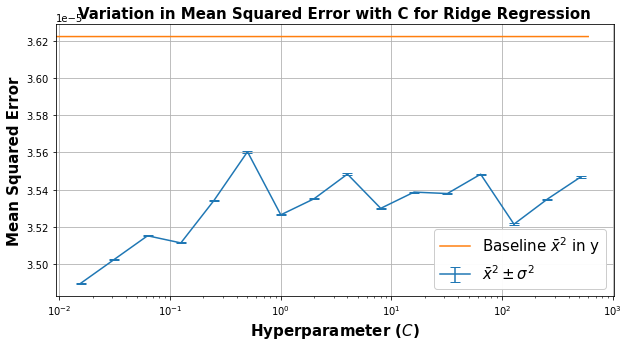
\includegraphics[width=0.8\linewidth]{pics/Ridge_MSE.png}
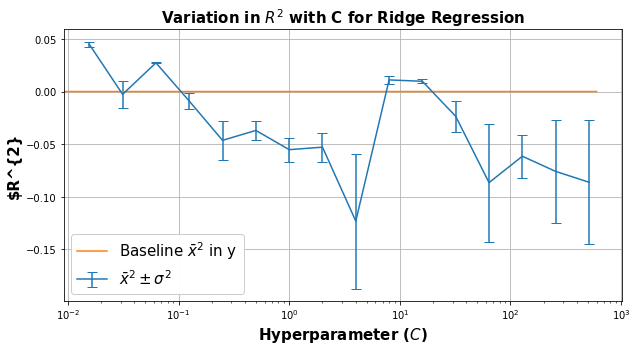
\includegraphics[width=0.8\linewidth]{pics/Ridge_R2.png}
\caption{Increasing C has a negative impact on MSE rather quickly, but the trend is much more difficult to discern for $R^2$.}
\label{fig:fig2}
\end{small}
\end{figure}

%PUT RESULTS FOR KNN HERE

\section{Discussion}

%Will's Graph Analysis
A high value for the optimal C was obtained in the experiment, at $65536$. The reason that this C value is so high lies in the way the LASSO method works; in minimising so many coefficients, the model fails to capture the significance of the data early on, only starting to have non-zero coefficients about C=1000. Ultimately, as the comparison is against the test data, it can safely be concluded that the model does not suffer from overfitting.

Comparatively, the Ridge regression achieves optimal results at a much lower value of C = 0.03125 as the coefficients, though small are not collectively minimised. If polynomial features were to have been appropriate for this dataset, perhaps the LASSO regression could have outperformed the Ridge regression, but no definitive remarks can be made.

%Darragh's part
One of the hyperparameters that was looked at was the addition of polynomial features. One key issue arose with this which was that due to the high number of parameters the program would run into a memory error, which meant that for this project, polynomial features would not be used.

%Will's part
The aforementioned method of target feature generation used the total number of reviews for a given game to weight the number of owners for a given game. This produced a source of bias towards games that received a higher number of either positive or negative reviews, giving more highly reviewed games more owners. This was deemed an acceptable trade-off against the fact that games may have more actual owners, but who do not leave reviews. As such, the number of owners used as the target feature also reflects the critical engagement of the owners.

\section{Summary}
Of all the models examined, Ridge regression proved to be the best predictor of the number of owners a videogame would have, based on data available prior to release. With an $R^2$ score of 0.127, it did perform above the baseline. This indicated that whilst the model was an improvement on the baseline, more refinement would be required to to produce a model worth releasing.

\section{Contributions}

\hspace{10pt} Darragh Hurley:\\

Code:
\begin{itemize}
    \item Reading in the json files
    \item Adding the genres to relevant games
    \item Combining all games into a single dictionary
    \item Attempted to run polynomial features as a hyperparameter
\end{itemize}

Report:
\begin{itemize}
    \item Part of dataset and features
    \item Part of discussion
\end{itemize}
%reading in the json files, adding the genres to relevant games and combining all games into one large dictionary. Attempted to run polynomial features as a hyperparameter.
%Report contribution - Part of dataset and features, part of discussion

\vspace{16pt}

William O'Sullivan:\\

Code:
\begin{itemize}
    \item Production of the target feature, Y
    \item Training and error analysis of LASSO and Ridge models
    \item Author of p\_model.py cells regarding training and graphing
\end{itemize}

Report:
\begin{itemize}
    \item introduction
    \item part of dataset and features regarding the target feature
    \item Methods
    \item Results of LASSO and Ridge Models
    \item Analysis of LASSO and Ridge results in discussion
    \item Analysis of target feature bias in discussion
\end{itemize}
%\\Code contribution - production of the target feature, Y. Training and error analysis of models as found in p\_model.py\\ Report contribution - Template, introduction, part of dataset and features regarding the target feature, methods, results, analysis of results in discussion, analysis of target feature in discussion.